\documentclass{headers/polimi_3i}

%------------------------------------------------------------------------------
%	REQUIRED PACKAGES AND  CONFIGURATIONS
%------------------------------------------------------------------------------

% CONFIGURATIONS
\usepackage{parskip} % For paragraph layout
\usepackage{setspace} % For using single or double spacing
\usepackage{emptypage} % To insert empty pages
\usepackage{multicol} % To write in multiple columns (executive summary)
\setlength\columnsep{15pt} % Column separation in executive summary
\setlength\parindent{0pt} % Indentation
\raggedbottom  

% PACKAGES FOR TITLES
\usepackage{titlesec}
% \titlespacing{\section}{left spacing}{before spacing}{after spacing}
\titlespacing{\section}{0pt}{3.3ex}{2ex}
\titlespacing{\subsection}{0pt}{3.3ex}{1.65ex}
\titlespacing{\subsubsection}{0pt}{3.3ex}{1ex}
\usepackage{color}

% PACKAGES FOR LANGUAGE AND FONT
\usepackage[english]{babel} % The document is in English  
\usepackage[utf8]{inputenc} % UTF8 encoding
\usepackage[T1]{fontenc} % Font encoding
\usepackage[11pt]{moresize} % Big fonts

% PACKAGES FOR IMAGES
\usepackage{graphicx}
\usepackage{transparent} % Enables transparent images
\usepackage{eso-pic} % For the background picture on the title page
\usepackage{subfig} % Numbered and caption subfigures using \subfloat.
\usepackage{tikz} % A package for high-quality hand-made figures.
\usetikzlibrary{}
\graphicspath{{./images/}} % Directory of the images
\usepackage{caption} % Coloured captions
\usepackage{xcolor} % Coloured captions
\usepackage{amsthm,thmtools,xcolor} % Coloured "Theorem"
\usepackage{float}

% STANDARD MATH PACKAGES
\usepackage{amsmath}
\usepackage{amsthm}
\usepackage{amssymb}
\usepackage{amsfonts}
\usepackage{bm}
\usepackage[overload]{empheq} % For braced-style systems of equations.
\usepackage{fix-cm} % To override original LaTeX restrictions on sizes

% PACKAGES FOR TABLES
\usepackage{tabularx}
\usepackage{longtable} % Tables that can span several pages
\usepackage{colortbl}

% PACKAGES FOR ALGORITHMS (PSEUDO-CODE)
\usepackage{algorithm}
\usepackage{algorithmic}

% PACKAGES FOR REFERENCES & BIBLIOGRAPHY
\usepackage[colorlinks=true,linkcolor=black,anchorcolor=black,citecolor=black,filecolor=black,menucolor=black,runcolor=black,urlcolor=black]{hyperref} % Adds clickable links at references
\usepackage{cleveref}
%\usepackage[square, numbers, sort&compress]{natbib} % Square brackets, citing references with numbers, citations sorted by appearance in the text and compressed
%\bibliographystyle{abbrvnat} % You may use a different style adapted to your field

% OTHER PACKAGES
\usepackage{pdfpages} % To include a pdf file
\usepackage{afterpage}
\usepackage{lipsum} % DUMMY PACKAGE
\usepackage{fancyhdr} % For the headers
\fancyhf{}

% Input of configuration file. Do not change config.tex file unless you really know what you are doing. 
% Define blue color typical of polimi
\definecolor{bluepoli}{cmyk}{0.4,0.1,0,0.4}

% Custom theorem environments
\declaretheoremstyle[
  headfont=\color{bluepoli}\normalfont\bfseries,
  bodyfont=\color{black}\normalfont\itshape,
]{colored}

% Set-up caption colors
\captionsetup[figure]{labelfont={color=bluepoli}} % Set colour of the captions
\captionsetup[table]{labelfont={color=bluepoli}} % Set colour of the captions
\captionsetup[algorithm]{labelfont={color=bluepoli}} % Set colour of the captions

\theoremstyle{colored}
\newtheorem{theorem}{Theorem}[chapter]
\newtheorem{proposition}{Proposition}[chapter]

% Enhances the features of the standard "table" and "tabular" environments.
\newcommand\T{\rule{0pt}{2.6ex}}
\newcommand\B{\rule[-1.2ex]{0pt}{0pt}}

% Pseudo-code algorithm descriptions.
\newcounter{algsubstate}
\renewcommand{\thealgsubstate}{\alph{algsubstate}}
\newenvironment{algsubstates}
  {\setcounter{algsubstate}{0}%
   \renewcommand{\STATE}{%
     \stepcounter{algsubstate}%
     \Statex {\small\thealgsubstate:}\space}}
  {}

% New font size
\newcommand\numfontsize{\@setfontsize\Huge{200}{60}}

% Title format: chapter
\titleformat{\chapter}[hang]{
\fontsize{50}{20}\selectfont\bfseries\filright}{\textcolor{bluepoli} \thechapter\hsp\hspace{2mm}\textcolor{bluepoli}{|   }\hsp}{0pt}{\huge\bfseries \textcolor{bluepoli}
}

% Title format: section
\titleformat{\section}
{\color{bluepoli}\normalfont\Large\bfseries}
{\color{bluepoli}\thesection.}{1em}{}

% Title format: subsection
\titleformat{\subsection}
{\color{bluepoli}\normalfont\large\bfseries}
{\color{bluepoli}\thesubsection.}{1em}{}

% Title format: subsubsection
\titleformat{\subsubsection}
{\color{bluepoli}\normalfont\large\bfseries}
{\color{bluepoli}\thesubsubsection.}{1em}{}

% Shortening for setting no horizontal-spacing
\newcommand{\hsp}{\hspace{0pt}}

\makeatletter
% Renewcommand: cleardoublepage including the background pic
\renewcommand*\cleardoublepage{%
  \clearpage\if@twoside\ifodd\c@page\else
  \null
  \AddToShipoutPicture*{\BackgroundPic}
  \thispagestyle{empty}%
  \newpage
  \if@twocolumn\hbox{}\newpage\fi\fi\fi}
\makeatother

%For correctly numbering algorithms
\numberwithin{algorithm}{chapter}

%----------------------------------------------------------------------------
%	NEW COMMANDS DEFINED
%----------------------------------------------------------------------------

%----------------------------------------------------------------------------
%	ADD YOUR PACKAGES (be careful of package interaction)
%----------------------------------------------------------------------------

\usepackage{enumitem}

\usepackage[style=numeric, sorting=nyt]{biblatex}

\addbibresource{chapters/biblio.bib}

%----------------------------------------------------------------------------
%	ADD YOUR DEFINITIONS AND COMMANDS (be careful of existing commands)
%----------------------------------------------------------------------------

%todo box highlight
\newcommand{\TODO}[1]{\noindent\colorbox{orange}{
	\parbox{\dimexpr\linewidth-2\fboxsep}
	{\textcolor{black}{\textbf{TODO:} #1}}}\par}

% Define a custom command for the list inside a table
% inserts padding on top and bottom, and no left indentation
\newcommand{\customtablelist}[1]{%
	\noindent
	\begin{minipage}[c]{6cm}
		\raggedright
		\begin{itemize}[left=0pt, after=\strut, before=\vskip 8pt]
			#1
		\end{itemize}
	\end{minipage}
}

\hyphenation{Interpret-ability}

%----------------------------------------------------------------------------
%	BEGIN OF YOUR DOCUMENT
%----------------------------------------------------------------------------

\begin{document}

\fancypagestyle{plain}{%
\fancyhf{} % Clear all header and footer fields
\fancyhead[RO,RE]{\thepage} %RO=right odd, RE=right even
\renewcommand{\headrulewidth}{0pt}
\renewcommand{\footrulewidth}{0pt}}




\startpreamble
\setcounter{page}{1} % Set page counter to 1
\addtocontents{toc}{\vspace{2em}} % Add a gap in the Contents, for aesthetics
\mainmatter % Begin numeric (1,2,3...) page numbering


\chapter{Robotic Platform for Mobile Manipulation}

This chapter will describe the robotic platform used for the project, specifically the hardware components.
The platform is composed of a mobile robot base, a robotic arm manipulator, sensors and perception systems, 
a soft gripper actuator, 3D-printed mounts, batteries, power management systems, and other electronic devices.
The chapter will also discuss the issues faced during the development of the mobile manipulation platform.

\section{Mobile Robot Platform}

The mobile robot used for the Thesis project is an \textit{AgileX Scout 2.0} robot, depicted in \ref{fig:c3_img01}.
This robot is a skid-steering robot, suitable for outdoor and indoor environments. 
Designed for robotics research and development, the Scout 2.0 is an unmanned ground vehicle (UGV). 
This autonomous mobile robot is CE-certified and offers a robust mechanical design along with capable mobility performance. 
Built to endure diverse conditions, Scout 2.0 features rugged materials and protective casings, ensuring longevity
and reliability during missions. SCOUT 2.0 offers aluminum T-slot rails for secure mounting of external sensors or kits. 
On these rails, a variety of sensors, computers, or other devices are mounted, allowing the creation of a mobile robotic platform
for a wide range of applications, and without relying on power cables to the wall, thanks to its 
\textbf{onboard battery system}.

It supports CAN bus protocol for connections and provides open-source SDK and software resources for expanded capabilities.
Its maximum speed is $1.5 m/s$, and it can carry a payload of $50$ kg. 
The robot is powered by a $24V$ battery, which provides a range of $15$ km maximum. 
The robot is controlled by a ROS-based software system, which allows the control of the robot's speed using a ROS topic
and receiving odometry data from the robot's encoders.

%Add the image of the robot
\begin{figure}[t]
	\centering
	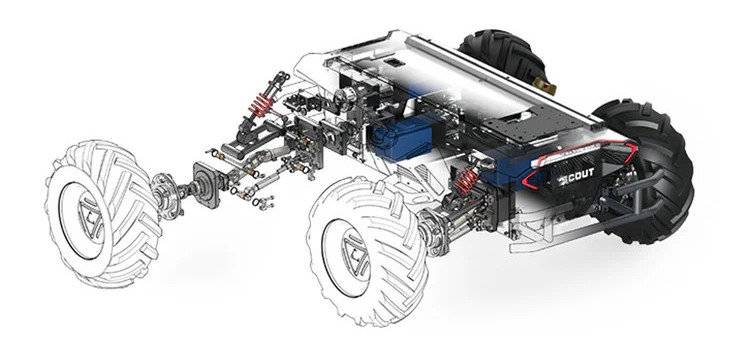
\includegraphics[width=1\textwidth]{chapter3_01.jpg}
	\captionsetup{width=1\linewidth}
	\caption{SCOUT employs 200W brushless servo motors to drive each wheel independently. 
    Its double-wishbone suspension with shock absorbers ensures stability on rough terrain, 
    enabling it to tackle obstacles up to 10cm tall effortlessly.}.
	\label{fig:c3_img01}
\end{figure}

On the mobile robot, an \textit{Intel NUC 12} computer \ref{fig:c3_img02} is mounted.
This \textbf{computer} is used for running all the control
software and the perception algorithms. The computer is connected to a switch, which is used to connect
the computer to the robot's control system and all the sensors and electronic devices mounted on the robot.
The computer is also connected to a router, which is used to connect the computer to the laboratory's network
and the internet. This allows the robot to be controlled remotely via a remote desktop connection.
This computer has the following technical specifications:

\begin{itemize}
    \item Intel Core i7-12700H CPU
    \item 32GB DDR4 RAM
    \item 1TB NVMe SSD
    \item Intel Iris Xe Graphics
    \item Kubuntu 22.04 operating system
\end{itemize}

% Add the image of the computer
\begin{figure}[t]
    \centering
    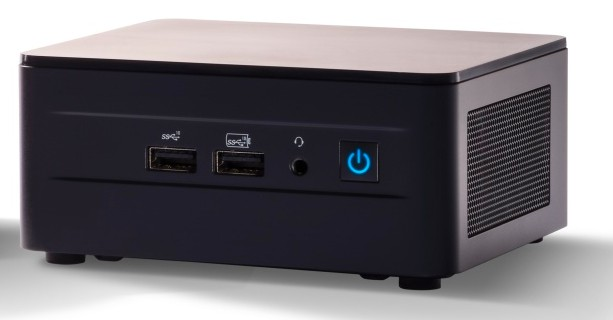
\includegraphics[width=0.6\textwidth]{chapter3_02.jpg}
    \captionsetup{width=1\linewidth}
    \caption{Intel NUC 12 computer mounted on the robot}.
    \label{fig:c3_img02}
\end{figure}

The robot is equipped with an \textit{TP-Link Archer MR200} router and a \textit{Netgear GS108} switch.
The router is used to connect the robot to the laboratory's network and the internet. The router was necessary to
establish a \textbf{remote connection} from a personal laptop to the robot's computer, allowing the control and monitoring
of the robot from a remote location. This was essential for the development of the project, as it allowed me to
work safely with the robot, ensuring that everything was working smoothly and stopping the system in case of any
unexpected behavior or software crashes and malfunctions.

The switch is used to connect the robot's computer to the robot's control system and all the sensors
and electronic devices mounted on the robot. The switch is connected to the router, allowing the robot's computer
to communicate with the laboratory's network and the internet. The robotic arm manipulator is also connected to the switch,
allowing the robot's computer to control the manipulator and receive data from its motors' encoders. 
The LiDAR is connected to the switch, allowing the robot's computer to receive pointcloud data from the LiDAR sensor,
at a fast transmission rate.
 
\section{Robotic Arm Manipulator}

The robotic arm manipulator used for the project is a \textit{Igus ReBeL 6-DoF} \textbf{cobot}, depicted in \ref{fig:c3_img04}.
Cobot is a term used to describe a collaborative robot, which is a robot designed to work alongside humans in a shared workspace.
This cobot is a lightweight, compact, and affordable robotic arm, suitable for research and development
in robotics. It is produced by the German company Igus, which specializes in the production of robotic components
for low-cost automation. The robotic arm is composed of six joints, each driven by a DC motor with an integrated encoder.
The outer contour and mechanical components of the ReBeL utilize Igus® plastic polymers, making it particularly inexpensive
and the lightest cobot on the market. Its lightweight and compact design makes it suitable for mounting on top
of mobile robot platforms, such as the Scout robot. The maximum payload of the arm is $2$ kg, which is more than enough
for the project's requirements. The weight is $8.2$ kg, which is light enough to be carried around by the mobile robot base,
without affecting the robot's mobility and stability.

The \textbf{advantages} of the ReBeL cobot are:

\begin{itemize}
    \item Lightweight, sleek and compact design
    \item Plastic arm, inexpensive and cost-effective
    \item Easy to install and operate with the provided software \ref{fig:c3_img05}
    \item Plug and play proprietary control system, or open-source control option
\end{itemize}

The \textbf{disadvantages} of the ReBeL cobot are:
\begin{itemize}
    \item Limited reach and workspace due to the joints' design and physical constraints
    \item Limited precision and repeatability
    \item The plastic gear components are not as durable and reliable as metal components
\end{itemize}

% Add the of the robotic arm
\begin{figure}[t]
    \centering
    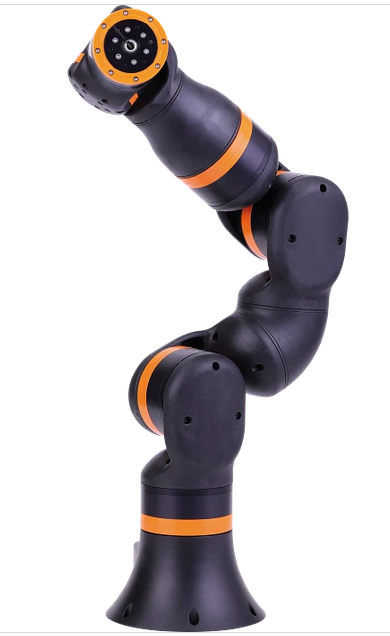
\includegraphics[width=0.3\textwidth]{chapter3_04.png}
    \captionsetup{width=1\linewidth}
    \caption{Igus ReBeL 6-DoF robotic arm (cobot)}.
    \label{fig:c3_img04}
\end{figure}

This robotic arm was the ideal choice for the project since the open-source control option allowed me to develop
the control software for the arm, based on ROS2 software packages. The lightweight and compact design made it suitable
for mounting on top of the SCOUT 2.0 robot, without affecting the robot's mobility and performance. 
The arm's easy installation and operation allowed me to quickly set up the arm and start developing the control software
and perception algorithms for the project.

% Add the image of the robotic arm software
\begin{figure}[t]
    \centering
    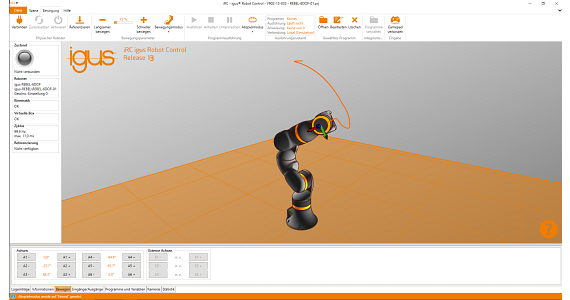
\includegraphics[width=0.8\textwidth]{chapter3_05.png}
    \captionsetup{width=1\linewidth}
    \caption{Igus ReBeL proprietary control software interface}.
    \label{fig:c3_img05}
\end{figure}

\subsection*{Issues with Igus Rebel motors' encoders and calibration}

Throughout the development of the project, I encountered several issues with the Igus ReBeL cobot.
The issues arose when the arm's motors' encoders were not providing accurate position data to the control software.
This caused the arm not to move to the defined joint positions with an accuracy of the end effector of $\pm 0.1mm$,
as specified by the manufacturer in the technical documentation.
This was mainly due to both the calibration of the motors' encoders and the plastic gear components' backlash and play.
The backlash and play in the gear components caused the arm's joints to have a certain amount of free movement before the motor
started to move the joint. This free movement caused the arm's joints to be in an incorrect position, which was not detected
by the motor's encoders. This resulted in the arm jiggling and vibrating when moving to a new joint position, and not reaching
the desired position with a smooth velocity profile.

Furthermore, the main issue encountered was the \textbf{calibration of the motors' encoders}.
This problem slowed down the development
of the project since the software solutions for the calibration of the encoders and the digital zeroing of the joints were not
successful in providing a working solution for the arm's accurate positioning. The calibration of the encoders was necessary
to provide accurate position data to the control software, allowing the arm to move to the desired joint positions with high
precision. The problem encountered was that the software for the automatic calibration of the motor controllers did not work
as expected, resulting in errors and faulty calibration of the encoders. The only solution was to replace the entire robot
arm with a new one, correctly calibrated by the manufacturer.

\section{Sensors and Perception}

The mobile robot platform is equipped with several sensors and perception systems, which are essential for the project's
objectives. The sensors and perception systems are used for mapping and localization, obstacle avoidance, object detection
and recognition, and manipulation tasks. 
Two main sensors are installed on the robot: a 3D LiDAR sensor and an RGB-D stereo camera sensor.
The LiDAR sensor is in a fixed position, on top of the robot to have a 360-degree field of view, while the camera sensor
is mounted on the robotic arm's wrist, allowing the camera to move with the arm's end effector.

\subsection{3D LiDAR Sensor}

The main sensor for environment perception for localization and navigation is mounted on the robot's T-slot rails.
The sensor is a \textit{Ouster OS1-64} LiDAR sensor, as shown in \ref{fig:c3_img06}.
The OS1 offers clean, dense data across its entire field of view for accurate perception and crisp detail in industrial,
automotive, robotics, and mapping applications.
This sensor is a \textbf{64-plane LiDAR sensor}, capable of providing a 360-degree field of view with a range of $120$ meters. 
The sensor has a resolution of $\pm 0.1cm$ and a stable scan rate of $10 Hz$ at $1024$ points resolution.
The vertical and horizontal scan resolution are $\pm 0.01$°.
Its minimum range of $0.5$ meters makes it suitable for indoor environments, while its maximum range of $120$ meters
makes it suitable also for outdoor environments.
This sensor was employed to create maps of the environments and also to localize the robot within the environment.
It proved also useful for dynamic obstacle avoidance, thanks to its high resolution and scan rate.

%insert image of the LiDAR sensor
\begin{figure}[t]
    \centering
    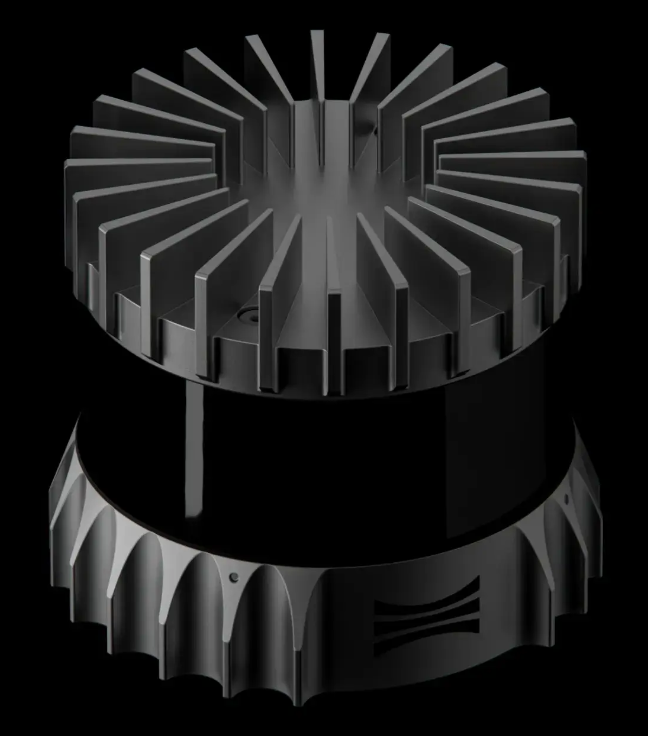
\includegraphics[width=0.5\textwidth]{chapter3_06.png}
    \captionsetup{width=1\linewidth}
    \caption{Ouster OS1-64 LiDAR sensor}.
    \label{fig:c3_img06}
\end{figure}

\subsection{RGB-D Stereo Camera Sensor}

The robotic arm is equipped with a \textit{Intel Realsense D435} RGB-D stereo camera sensor, shown in \ref{fig:c3_img07}.
This camera is mounted on the \textit{wrist} of the robotic arm, allowing the camera to move with the arm's end effector.
The camera is used for object detection and recognition, and also for Aruco markers detection and pose estimation.
This is the camera of choice for robotic applications, as it provides both RGB and depth images, which are essential
for perception tasks in robotics. The camera is also lightweight and compact, making it suitable for mounting on the cobot.

The Intel RealSense D435 is a stereo depth camera that is designed for capturing RGB and depth images.
The camera is equipped with a global shutter and a rolling shutter, which allows it to capture images with a resolution
of $1920\times1080$ pixels at $30$ frames per second, even though the ROS2 driver provided by Intel reduces the resolution
to $640\times480$ pixels at $30$ frames per second. The camera has a field of view of $85.2$° horizontal, $58$° vertical,
and $94$° diagonal. The depth camera works within a range of $0.3$ meters to $3$ meters while maintaining 
high accuracy and precision.

% Add an image of the camera
\begin{figure}[t]
    \centering
    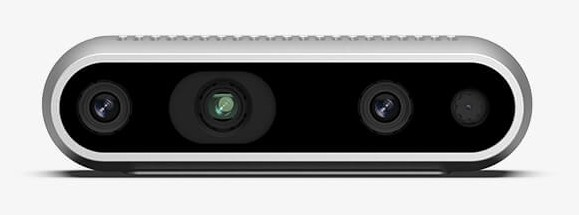
\includegraphics[width=0.5\textwidth]{chapter3_07.jpg}
    \captionsetup{width=1\linewidth}
    \caption{Intel RealSense D435 RGB-D stereo camera}.
    \label{fig:c3_img07}
\end{figure}

\subsection{Issues with Intel Realsense calibration}

The camera provided by the laboratory was not calibrated correctly, especially the depth estimations were not accurate.
In fact, the depth images provided depth estimations that were not consistent with the real-world distances of the objects
in the environment. I was able to discover such issues when I started using the camera's depth sensor for the perception
tasks of the project. I realized that the estimated distance from the camera and the Aruco markers (the distance estimated
using geometrical calculations and the camera's intrinsic parameters) was \textbf{not consistent} with the estimated distance
to the marker provided by the camera's depth sensor. This inconsistency was due to the camera's depth sensor not being
calibrated correctly.

% Add the image of the calibration pattern
\begin{figure}[t]
    \centering
    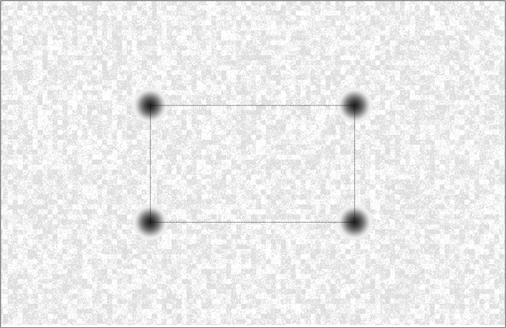
\includegraphics[width=0.5\textwidth]{chapter3_08.png}
    \captionsetup{width=1\linewidth}
    \caption{Calibration pattern used for the camera's depth image calibration}.
    \label{fig:c3_img08}
\end{figure}

This issue was critical for the project, as the depth sensor was used for many perception algorithms.
I managed to solve this issue by calibrating the camera's depth sensor using the proprietary software provided by Intel:
\textit{Interl Realsense Self-Calibration Tool}, an application for \textbf{automatic on-chip calibration}.
The calibration process was straightforward and required a few minutes to complete, even though many trials were needed
to find the best possible calibration parameters. Two calibration procedures were carried out:

\begin{itemize}
    \item \textbf{Intrinsic parameters calibration}: this calibration process was used to calibrate the camera's 
    intrinsic parameters,
    such as the focal length, principal point, and distortion coefficients. This calibration was necessary to correct
    the distortion of the images and to provide accurate depth estimations from the RGB sensor. The calibration process
    required the camera to capture a series of images of a calibration pattern (checkerboard pattern) from different angles
    and distances. The calibration software then used these images to estimate the intrinsic parameters of the camera.
    \item \textbf{Depth sensor calibration}: this calibration process required the camera to capture a series of
    depth images of a calibration sheet \ref{fig:c3_img08}, which was a flat surface with known distances between the points.
    The calibration software then used these depth images to estimate the depth sensor's parameters, 
    such as the depth scale factor and the depth offset. 
    These parameters were necessary to correct the depth estimations of the camera's depth sensor.
\end{itemize}


After the calibration process, the camera's depth sensor was providing accurate and consistent depth estimations,
which were consistent with the real-world distances of the objects in the environment.

\section{Soft Gripper Actuator}

The robotic arm is equipped with a Soft Gripper Pneumatic Actuator from \textit{Soft Gripping}, depicted in \ref{fig:c3_img09}.
This gripper is composed of 3 soft fingers, which are actuated by a pneumatic pump. The fingers are made of
\textbf{silicone rubber}, which is soft and flexible, allowing the gripper to grasp and manipulate objects of different shapes
and sizes. The silicone material of the fingers is also non-slip, which ensures a secure grip on the objects.
It is also essential in food industries, where the gripper is used to handle delicate and fragile objects, 
such as fruits. The other advantage is that silicone is non-toxic and food-safe, making it suitable for handling
food products.

% Add the image of the soft gripper
\begin{figure}[t]
    \centering
    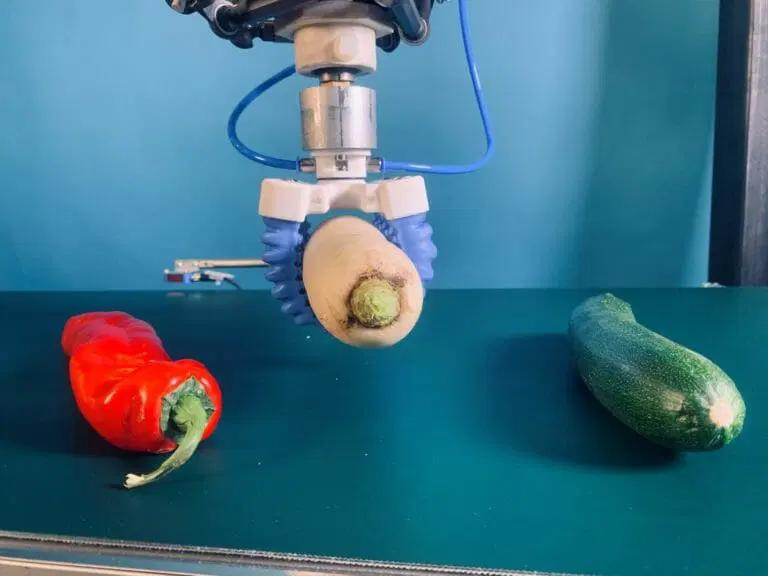
\includegraphics[width=0.6\textwidth]{chapter3_09.jpg}
    \captionsetup{width=1\linewidth}
    \caption{Soft Gripper Pneumatic Actuator handling vegetables}.
    \label{fig:c3_img09}
\end{figure}

The soft gripper is controlled by a pneumatic pump \ref{fig:c3_img13}, which provides compressed air to the fingers,
allowing them to open and close. The pneumatic system works at a pressure of $1$ bar when the fingers are closed, and at
a negative pressure of $0$ bar when the fingers are opened. The pneumatic pump that controls the soft gripper
allows the user to set the pressure value used when closing the fingers, but the pressure value cannot be
changed dynamically via electronic control. Figure \ref{fig:sg_combined} shows the soft gripper mounted on the end effector
with the fingers opened and closed.

% Add a picture of the pneumatic pump
\begin{figure}[t]
    \centering
    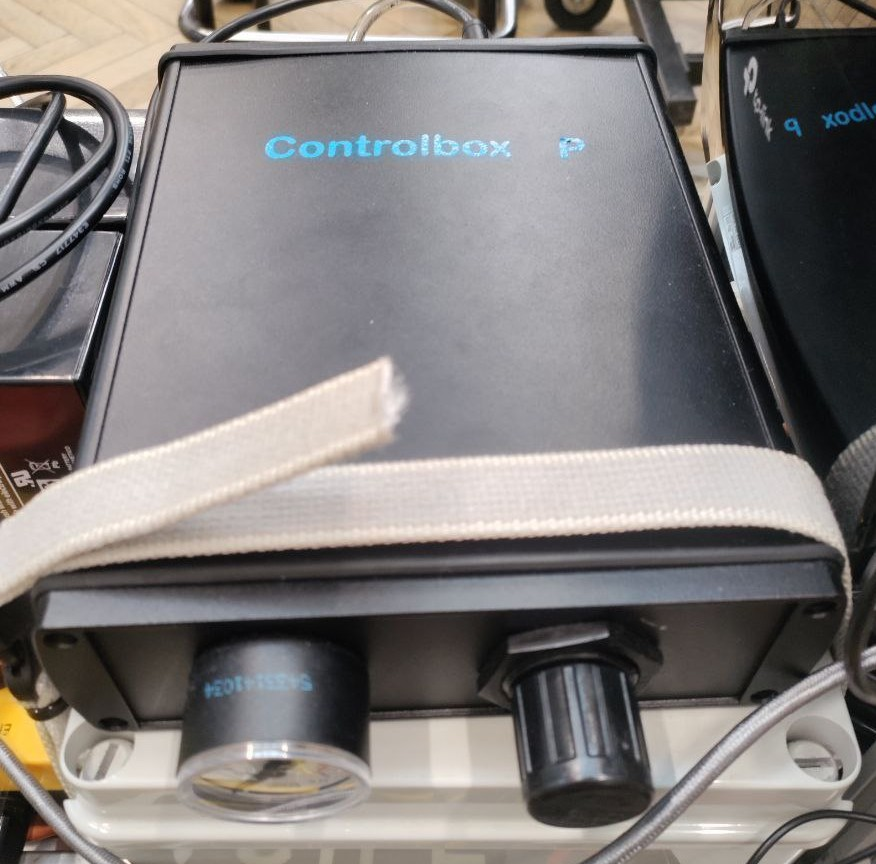
\includegraphics[width=0.6\textwidth]{c3_13.jpg}
    \captionsetup{width=1\linewidth}
    \caption{Pneumatic Pump control box secured on top of the mobile robot}.
    \label{fig:c3_img13}
\end{figure}

The pneumatic pump provided with the soft gripper has only one output tube used for providing positive pressure
to the fingers. The negative pressure is provided by the environment, as the fingers are opened by the air pressure
inside the fingers, which is lower than the air pressure outside the fingers. 
Other versions of the pneumatic pump provide also a negative pressure output tube, which allows the user to control
the pressure value used when opening the fingers, but this feature requires an external vacuum compressor to work.

The gripper is mounted on the robotic arm's end effector, allowing the arm to grasp and manipulate
objects in the environment. It is placed strategically close to the robotic arm's flange to ensure
that the mobility and reach of the end effector are not affected by the gripper's size.
Furthermore, the soft gripper is very lightweight and compact, making it suitable for mounting on the cobot.

% Add pictures of the gripper opened and closed
\begin{figure}[t]
    \centering
    \begin{subfigure}{0.45\textwidth}
        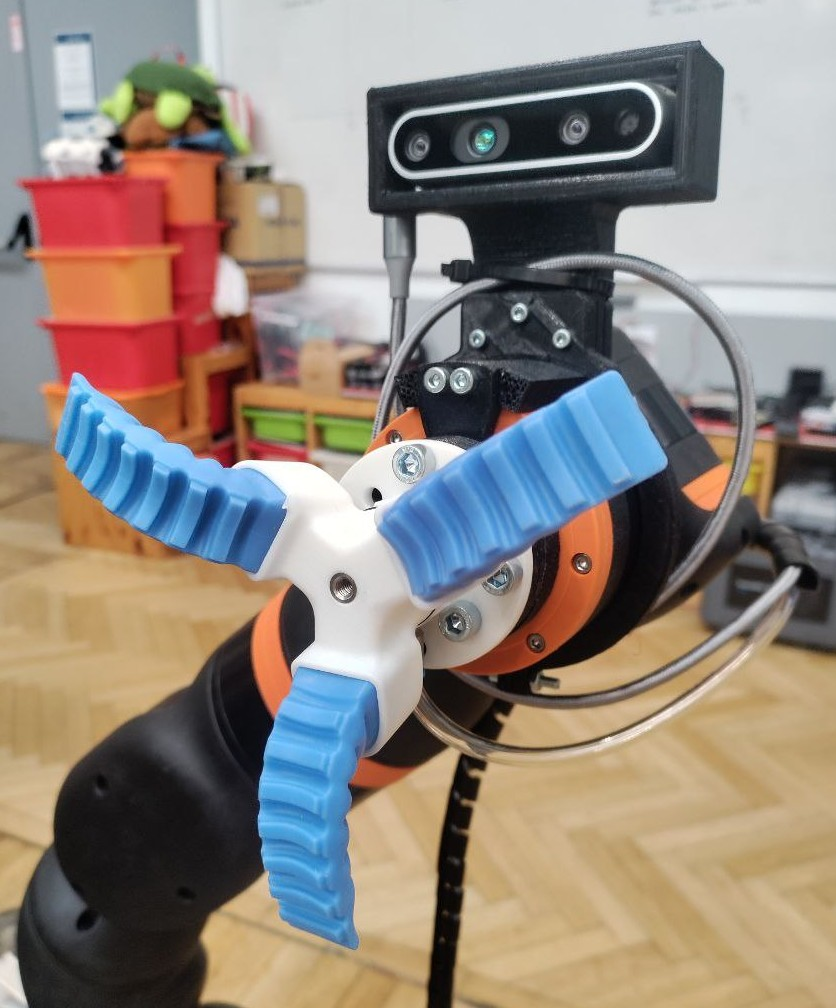
\includegraphics[width=1\textwidth]{c3_26.jpg}
        \caption{Soft Gripper opened}
        \label{fig:opened}
    \end{subfigure}
    \hfill % Optional: Adds space between images
    \begin{subfigure}{0.45\textwidth}
        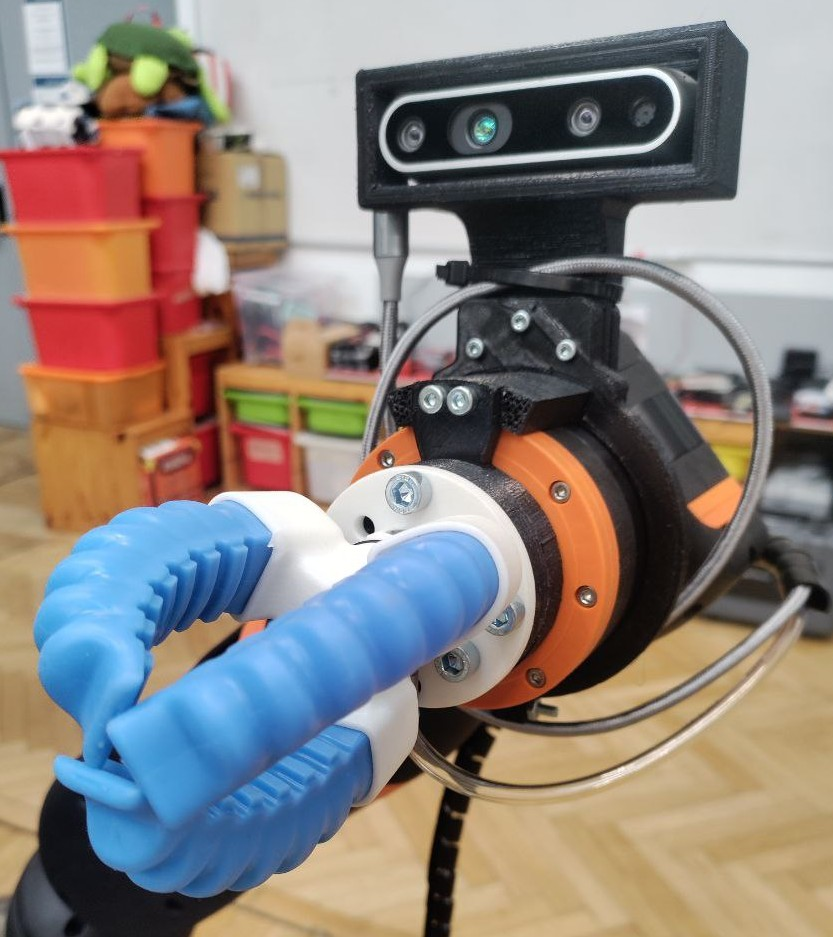
\includegraphics[width=1.07\textwidth]{c3_25.jpg}
        \caption{Soft Gripper closed}
        \label{fig:closed}
    \end{subfigure}
    \caption{Soft Gripper mounted on the end effector}
    \label{fig:sg_combined}
\end{figure}

The pneumatic pump is provided without any power supply, so it was necessary to create a system to power the pump
using the \textbf{onboard batteries}. The pump is powered by a 24V lead battery, which is the same battery powering
the robotic arm. I created a system for powering both the robotic arm and the pneumatic pump with the same battery,
using Molex cables and connectors. These Molex cables proved to be a reliable and optimal solution,
as they allowed me to switch easily between the onboard batteries and the external cobot power supply.
The Molex cable management is shown in \ref{fig:c3_img12}.
In fact, the cobot's power supply provides 24V at a maximum of 10A, which is enough to power the robotic arm
and the pneumatic pump simultaneously, since the pneumatic pump doesn't require a high current to operate.
The cable of the external power supply is also a Molex cable, so that's why I used Molex connectors and cables
to connect the robotic arm and the pneumatic pump to the cobot's power supply.

% Add a picture of the Molex connectors and cables
\begin{figure}[t]
    \centering
    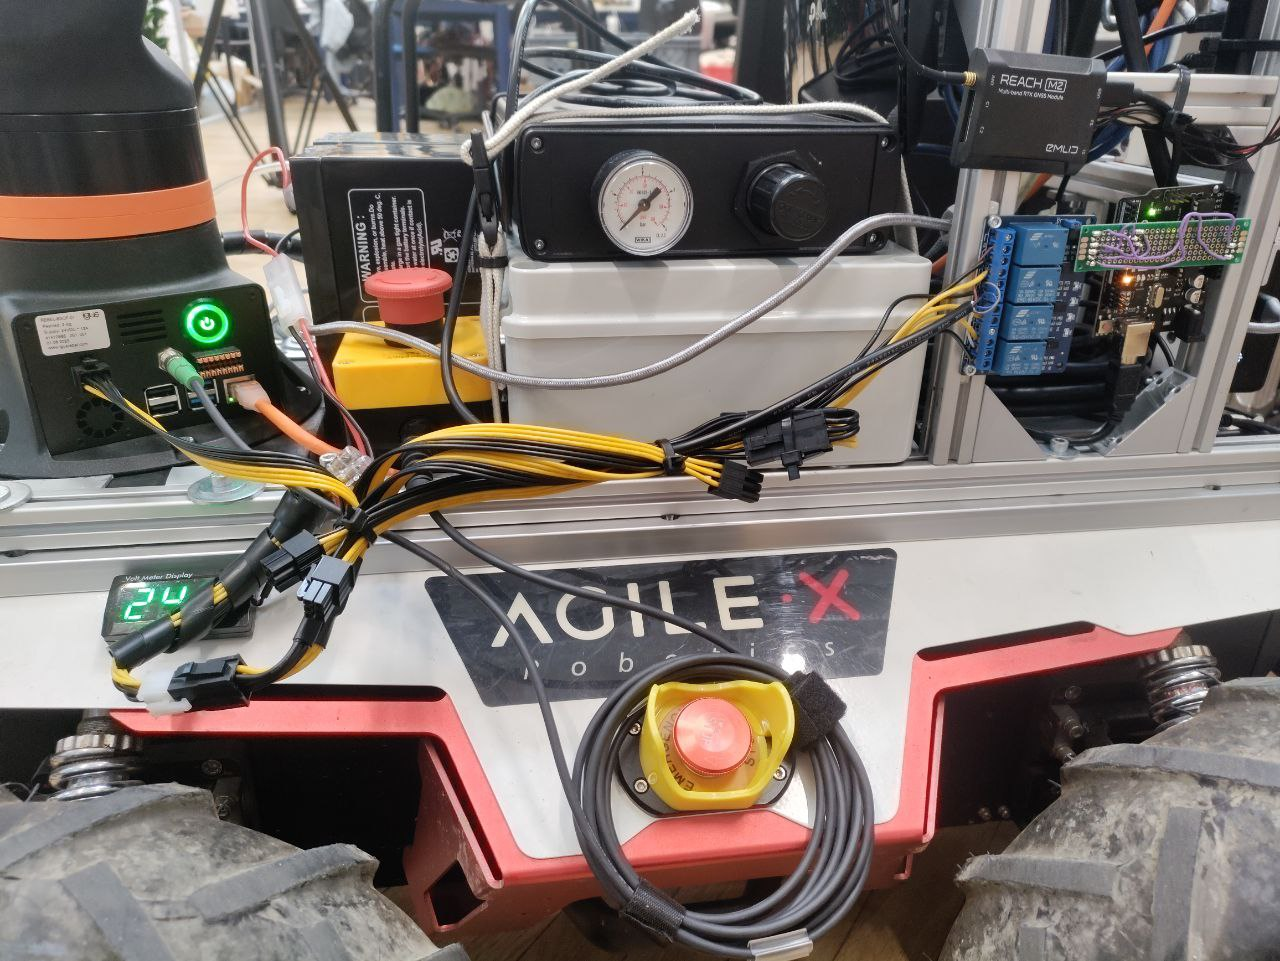
\includegraphics[width=0.6\textwidth]{c3_12.jpg}
    \captionsetup{width=1\linewidth}
    \caption{Molex connectors and power management for the cobot, pump, and relays}.
    \label{fig:c3_img12}
\end{figure}

The pneumatic pump must be controlled at 24V, as the pump's solenoid valve requires this voltage to operate.
The pump provides 4 digital pins for controlling its operation, which are used to open and close the fingers.
I created a simple system capable of controlling the pump's operation using an \textbf{Arduino UNO microcontroller}.
The Arduino UNO is connected to the robot's computer via USB, allowing the computer to send commands to the Arduino
via the serial port. The Arduino UNO is then connected to the pneumatic pump via a relay module,
composed of 4 different relays, each controlling a different digital pin of the pump. The relays were necessary
to provide an output voltage of 24V, while the Arduino UNO provides only 5V via its digital pinout.
The relays are cheap and quick enough to switch between the digital pins of the pump, allowing efficient
control of the pump's operation, and the installation of simple circuitry for the control system 
directly on the mobile robot platform. Figure \ref{fig:c3_img10} shows the Arduino UNO microcontroller
and the relay module used to control the pneumatic pump.

% Add a picture of the Arduino UNO and the relay module
\begin{figure}[t]
    \centering
    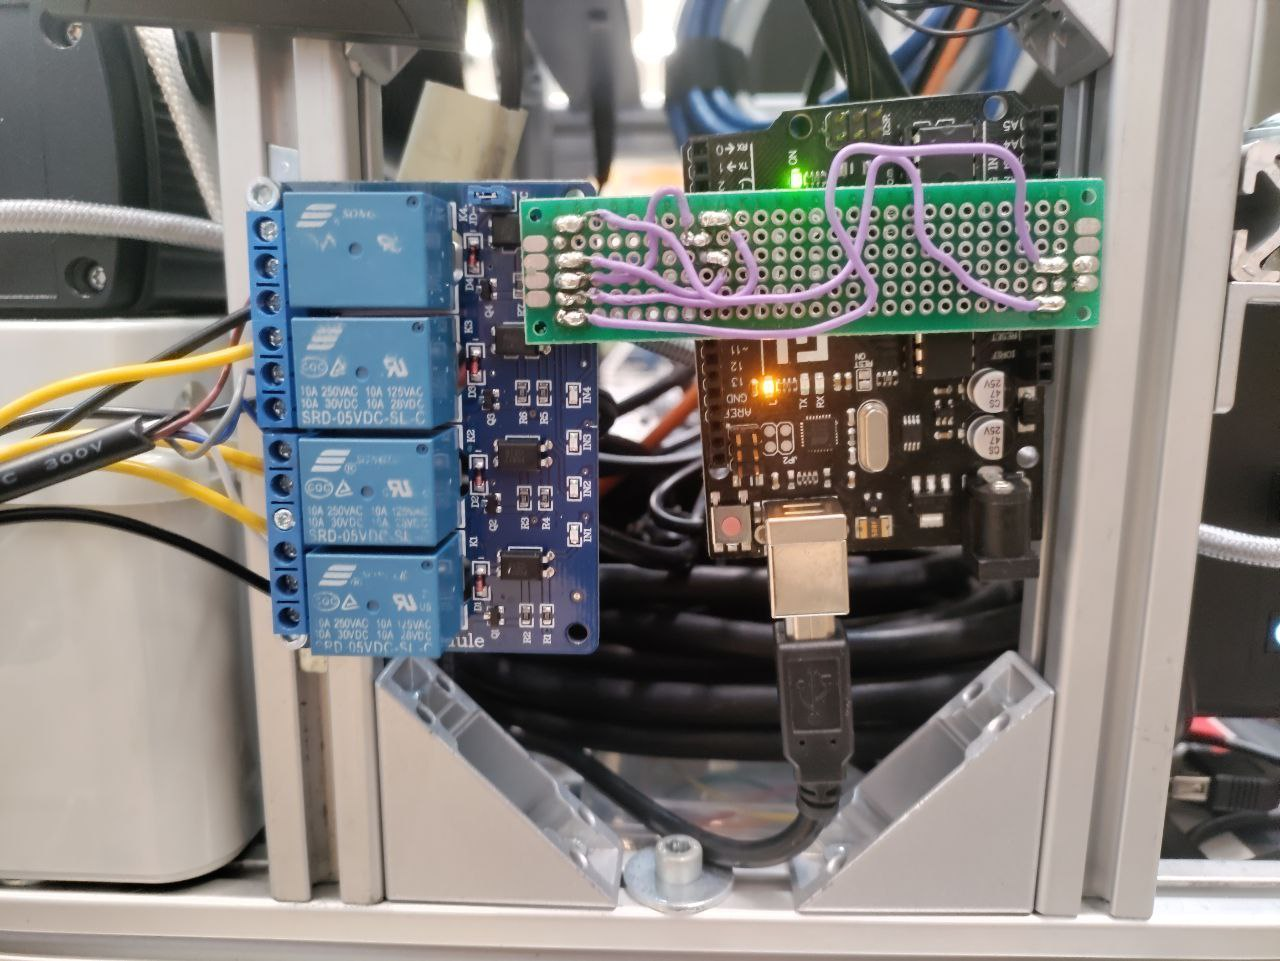
\includegraphics[width=0.6\textwidth]{c3_11.jpg}
    \captionsetup{width=1\linewidth}
    \caption{Arduino UNO microcontroller and relay module used to control the pneumatic pump}.
    \label{fig:c3_img10}
\end{figure}

\section{3D Printed Mounts Design}

Mounting the sensors and electronic devices on the mobile robot platform required the design and 3D printing
of custom mounts. The mounts were designed using the \textit{Fusion 360} CAD software, which allowed me to create
precise and accurate models of the mounts. The mounts were then 3D printed using the laboratory's 3D printer,
which is a \textit{Creality CR-10S} 3D printer. 

I designed and created the \textbf{mount for the GPS antenna}, which was used for outdoor localization
and navigation tasks. The GPS antenna mount was designed to be placed on top of the LiDAR sensor, ensuring
that the antenna had a clear view of the sky and the satellites. The mount was also designed to be lightweight
and quick to install, without affecting the LiDAR sensor's field of view, and without using any screws or bolts.
Figure \ref{fig:gpsprint} shows the mount installation on top of the LiDAR sensor, while Figure \ref{fig:gps3d}
shows the 3D design of the mount.
I never used the GPS in my project, but the support that I created for it was used by other researchers 
in the laboratory for other projects.

% Add pictures of the GPS antenna mount render and 3D print
\begin{figure}[t]
    \centering
    \begin{subfigure}{0.3\textwidth}
        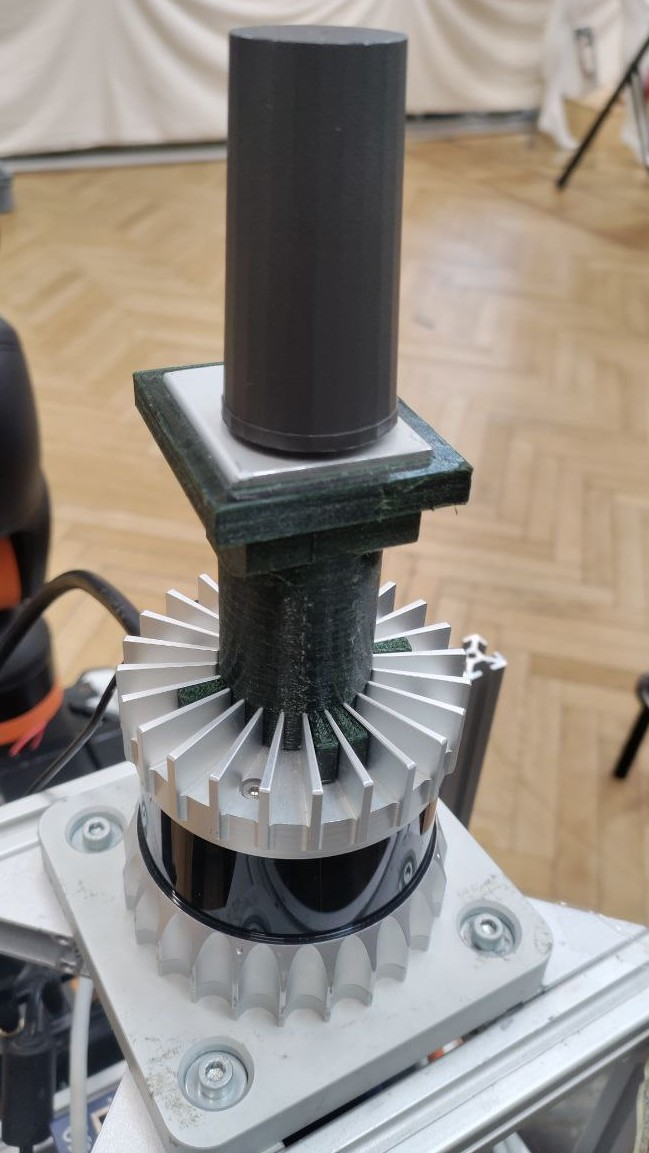
\includegraphics[width=0.7\textwidth]{c3_20.jpg}
        \captionsetup{width=0.9\linewidth}
        \caption{GPS antenna 3D-printed mount}
        \label{fig:gps3d}
    \end{subfigure}
    \hfill
    \begin{subfigure}{0.67\textwidth}
        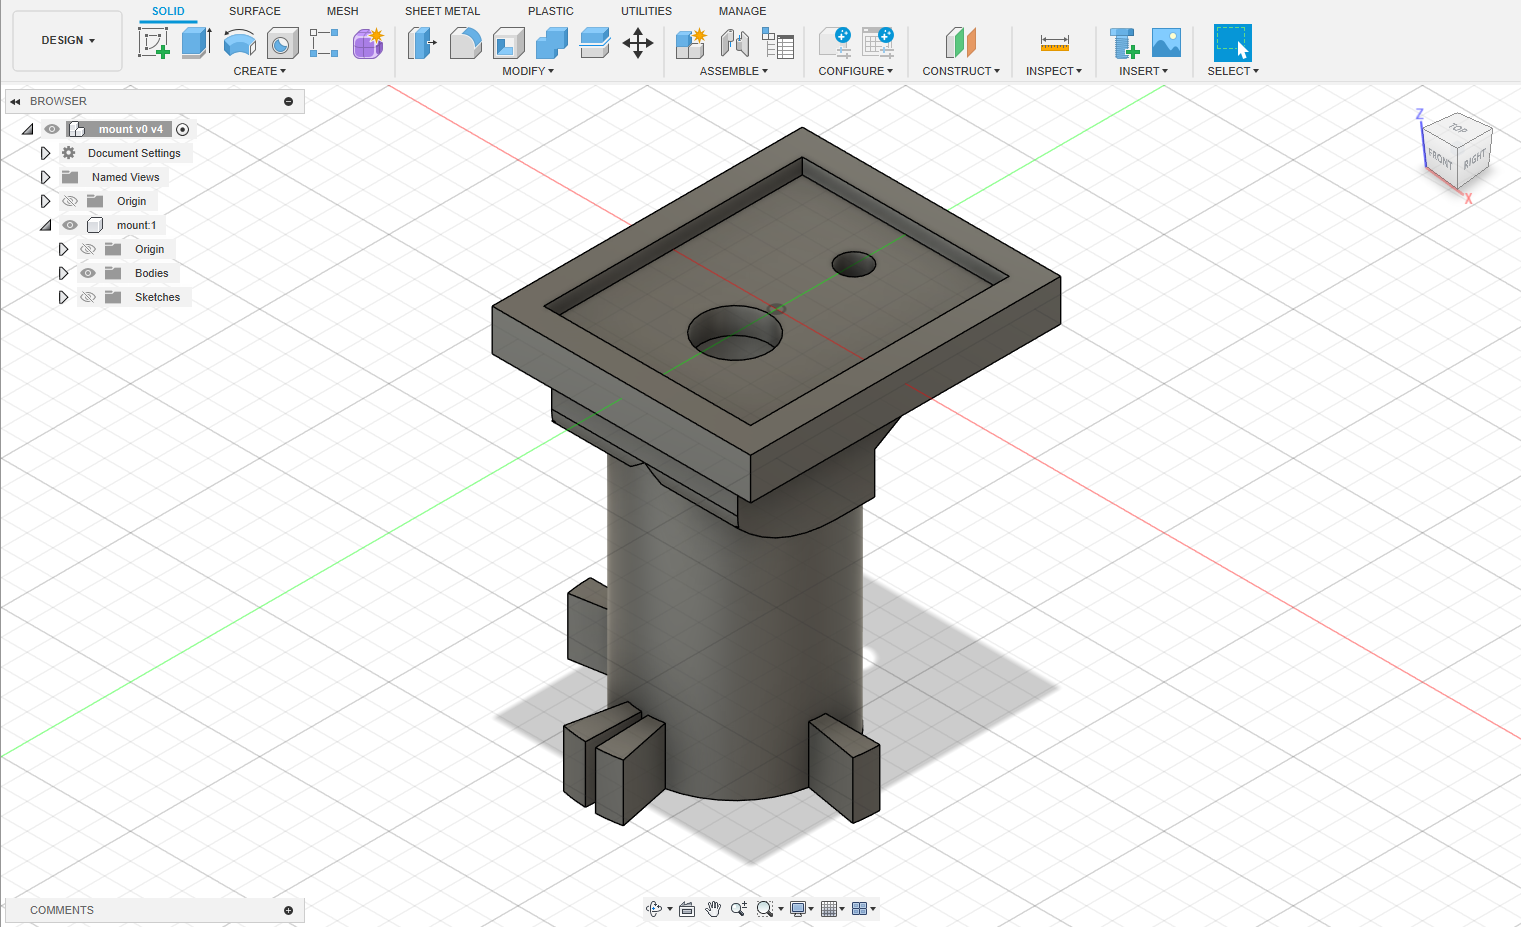
\includegraphics[width=1.0\textwidth]{c3_22.png}
        \caption{3D design}
        \label{fig:gpsprint}
    \end{subfigure}
    \captionsetup{width=1\linewidth}
    \caption{GPS antenna mount design and 3D-print on top of the LiDAR}.
    \label{fig:c3_gps}
\end{figure}

The 3D printer that I used in the AIRLab is a Fused Deposition Modeling (FDM) printer,
which uses a thermoplastic filament to create the 3D models layer by layer. The material of choice
for the 3D prints was \textit{PETG} (Polyethylene Terephthalate Glycol), which is a strong and durable material,
suitable for mechanical parts and mounts. The PETG material is also resistant to mechanical stress and heat,
making it the ideal material for the mounts for these kinds of applications.

I designed and printed two versions of the mount for the cobot's flange:

\begin{itemize}
    \item \textit{Mount V1} \ref{fig:mountv1}: a mount for the Realsense camera and a digital button on top of a cylinder used
    for pressing buttons on a control panel. The mount was designed to be robust and easy to switch with other
    mount extensions. This mount was used for the first demos and tests of the project.
    \item \textit{Mount V2} \ref{fig:mountv2}: a mount for the Realsense camera and the soft gripper as an end-effector.
    This mount was designed to be compact, robust, and more effective for the final versions of the project.
\end{itemize}

The 3D-printed mounts were designed to be lightweight and compact, to ensure that the robot's mobility and stability
were not affected. The mounts were also designed to be very robust and durable, to withstand the vibrations and shocks
of the mobile robot platform. The mounts are not very easy to install and remove, since they are designed to be
mounted with several screws and bolts, ensuring that the sensors and electronic devices are securely attached to the robot.
These mounts demonstrated to be very effective and reliable, as they withstood the vibrations while maintaining
the sensors in their fixed position.

\subsection{Mount V1}

% Add pictures of the Mount V1 render and 3D print
\begin{figure}
    \centering
    \begin{subfigure}{\textwidth}
        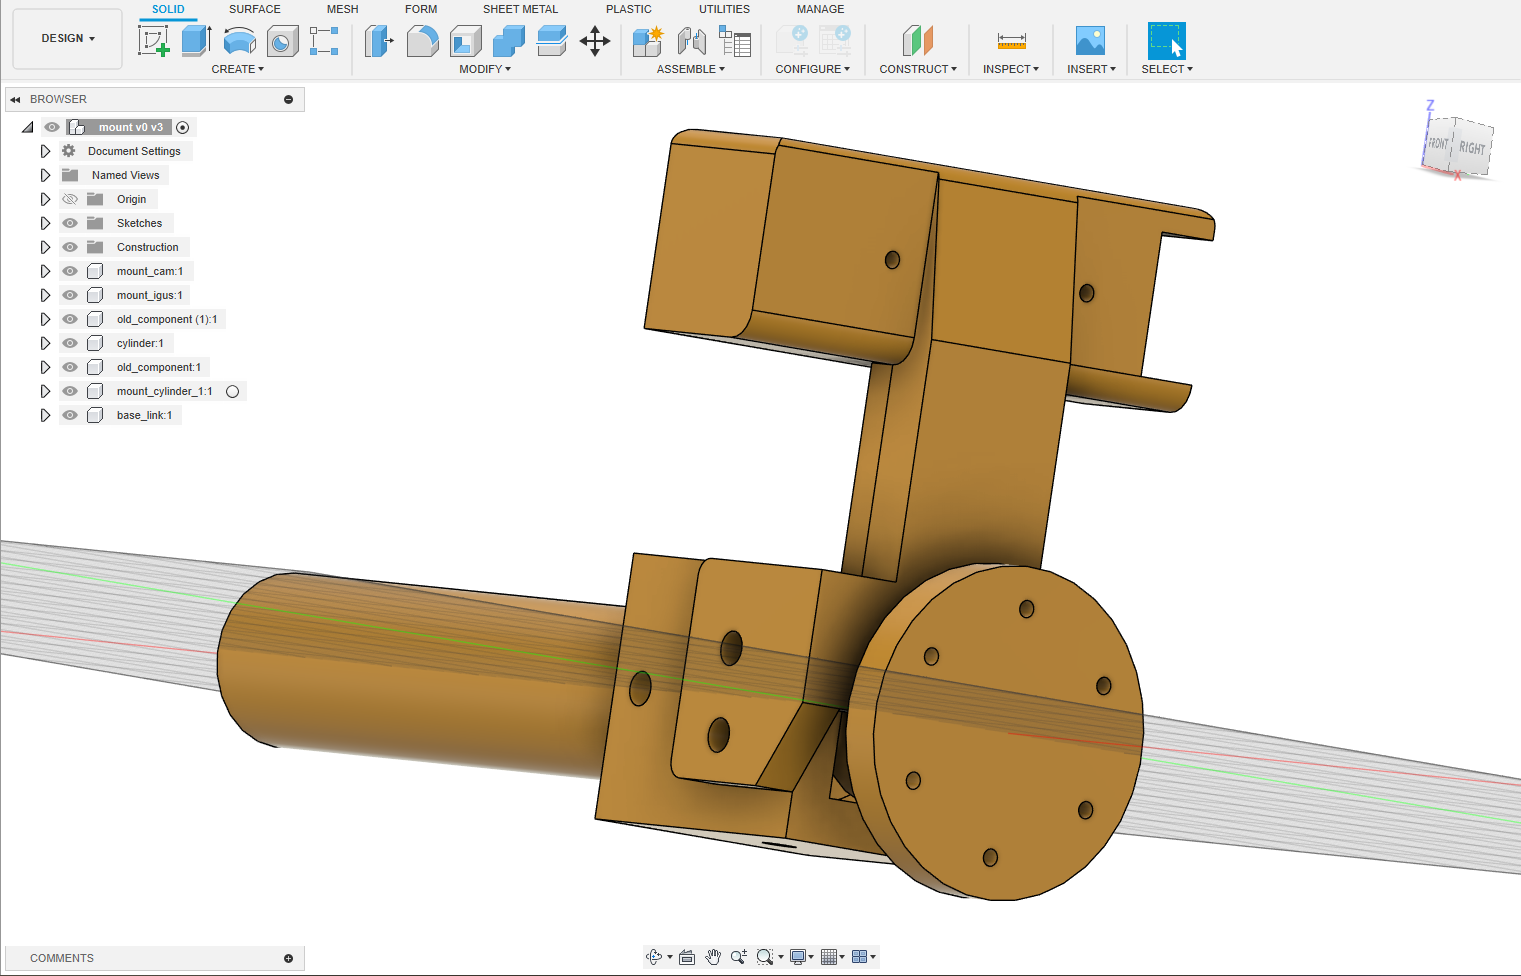
\includegraphics[width=0.9\textwidth]{c3_20.png} % Replace with your image file
        \caption{Back side view of the 3D design}
        \label{fig:frontv1}
    \end{subfigure}
    
    \vspace{1em} % Add some vertical space between images (adjust as needed)

    \begin{subfigure}{\textwidth}
        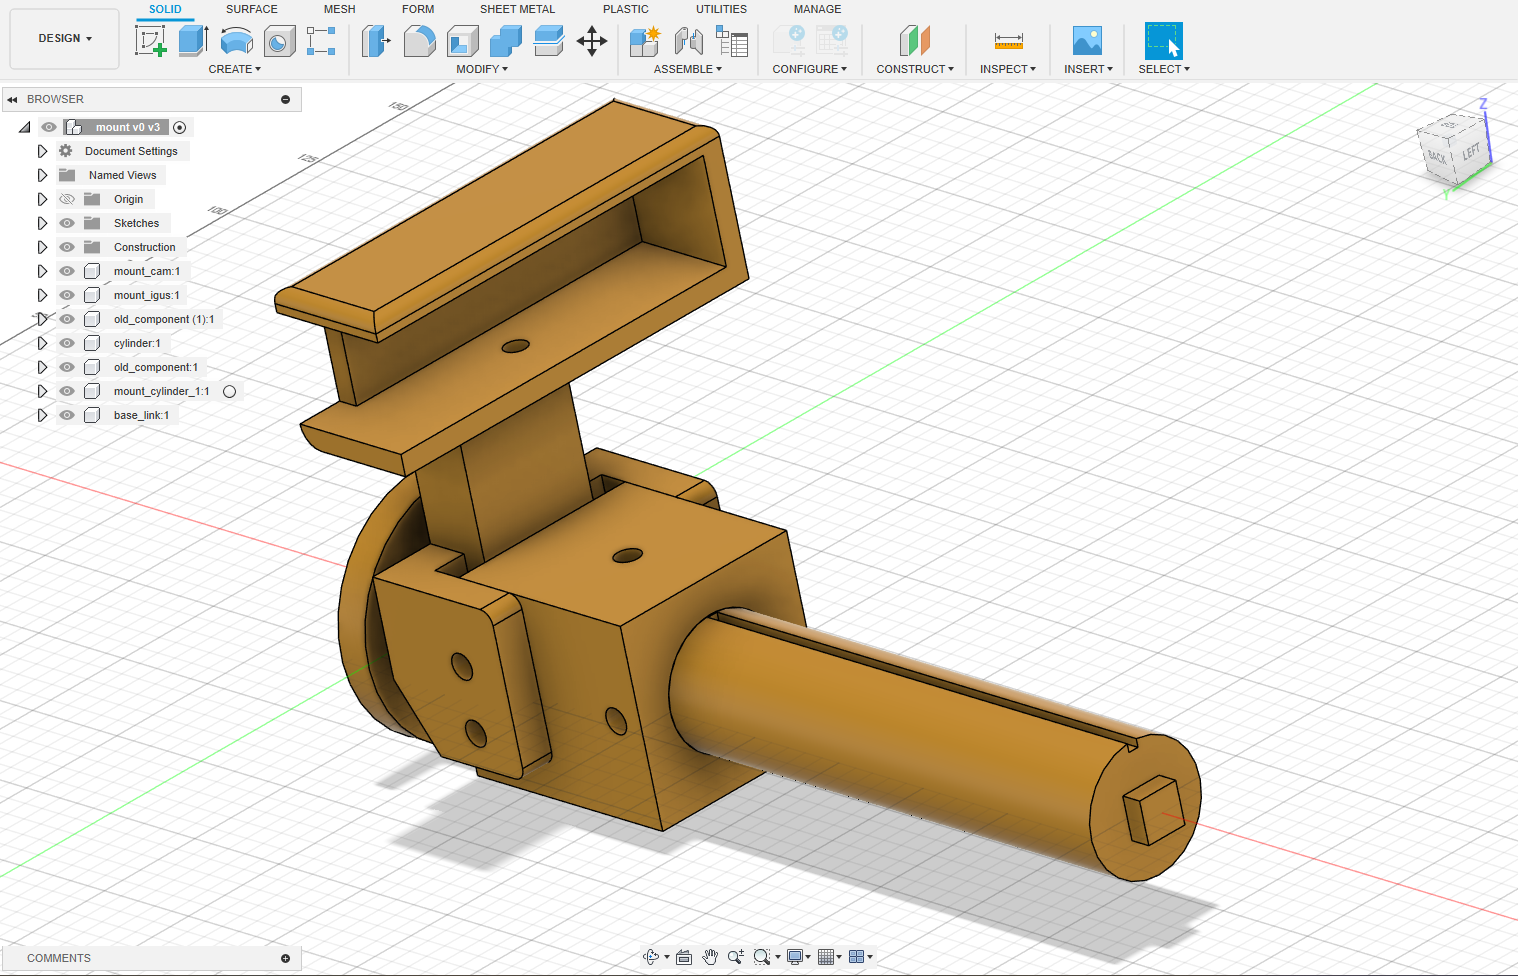
\includegraphics[width=0.9\textwidth]{c3_23.png} % Replace with your image file
        \caption{Frontal side view of the 3D design}
        \label{fig:sidev1}
    \end{subfigure}

    \caption{MountV1 Design screenshots from \textit{Autodesk Fusion 360}}
    \label{fig:mountv1}
\end{figure}

The first version of the mount, alias \textit{Mount V1}, shown in \ref{fig:mountv1},
was designed to be robust and easy to switch with other mount extensions. 
The mount was designed to be lightweight and long, to ensure that the cobot's end effector
would be able to reach objects not in the immediate vicinity of the robot. The mount was also designed to be
compact, with the stereo camera mounted in front of the cobot's flange, and the digital button mounted on top
of a cylinder used for pressing buttons on a control panel. The mount was also designed to be very robust and durable.

After many tests, the cylinder was then shrunk to a smaller length, to ensure that the cobot's end effector
mobility and reach were not affected negatively. This allowed the cobot's end effector to reach objects
in the vicinity with fewer limitations and constraints on its orientation.
The digital button placed on the tip was initially used as a digital feedback mechanism for the pressure
of the buttons on the control panel. This button was later removed, as it was not necessary for the project's
objectives. The mount was then used for the first demos and tests of the project, and it proved to be very effective.

One of the main issues encountered with the mount was the \textbf{reduced field of view of the stereo camera}, due to its
installation on the cobot's flange. The camera was placed at the right distance from the center of the cobot's flange,
making it possible for the camera's field of view not to be obstructed by the cylinder.
After many tests, I realized that the best configuration would be to mount the camera on top of the wrist,
to enlarge the field of view. The Mount V1 was used for the "button presser demo", and replaced with its 
second improved version for the next demos.

\subsection{Mount V2}

% Add pictures of the Mount V2 render and 3D print
\begin{figure}
    \centering

    \begin{subfigure}{\textwidth}
        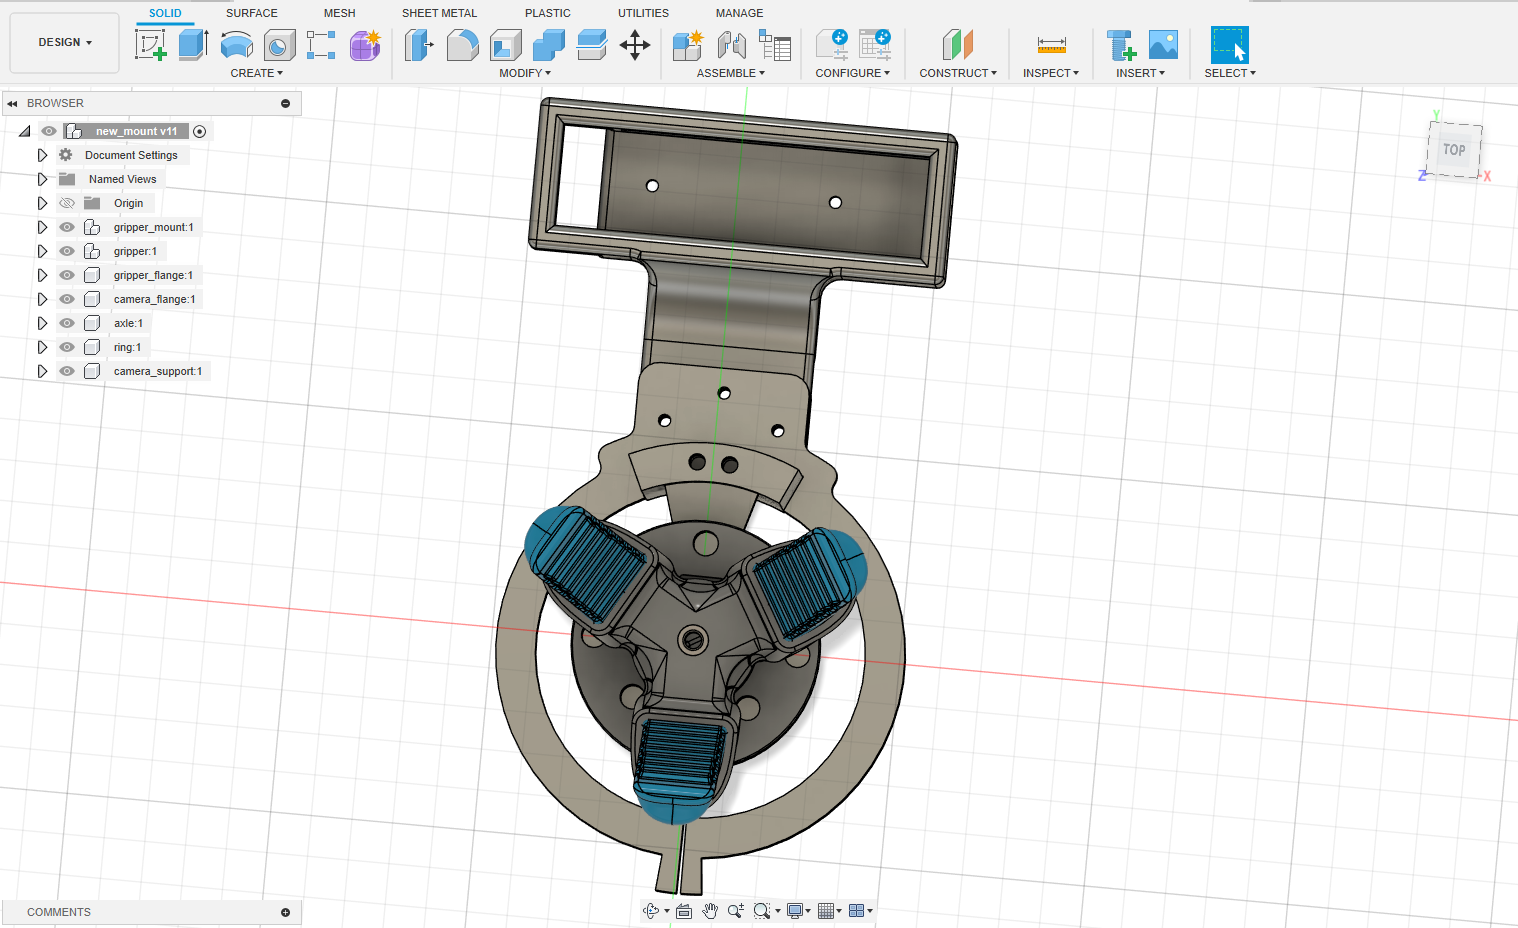
\includegraphics[width=\textwidth]{c3_21.png} % Replace with your image file
        \caption{Front view of the 3D design}
        \label{fig:frontv2}
    \end{subfigure}
    
    \vspace{1em} % Add some vertical space between images (adjust as needed)

    \begin{subfigure}{\textwidth}
        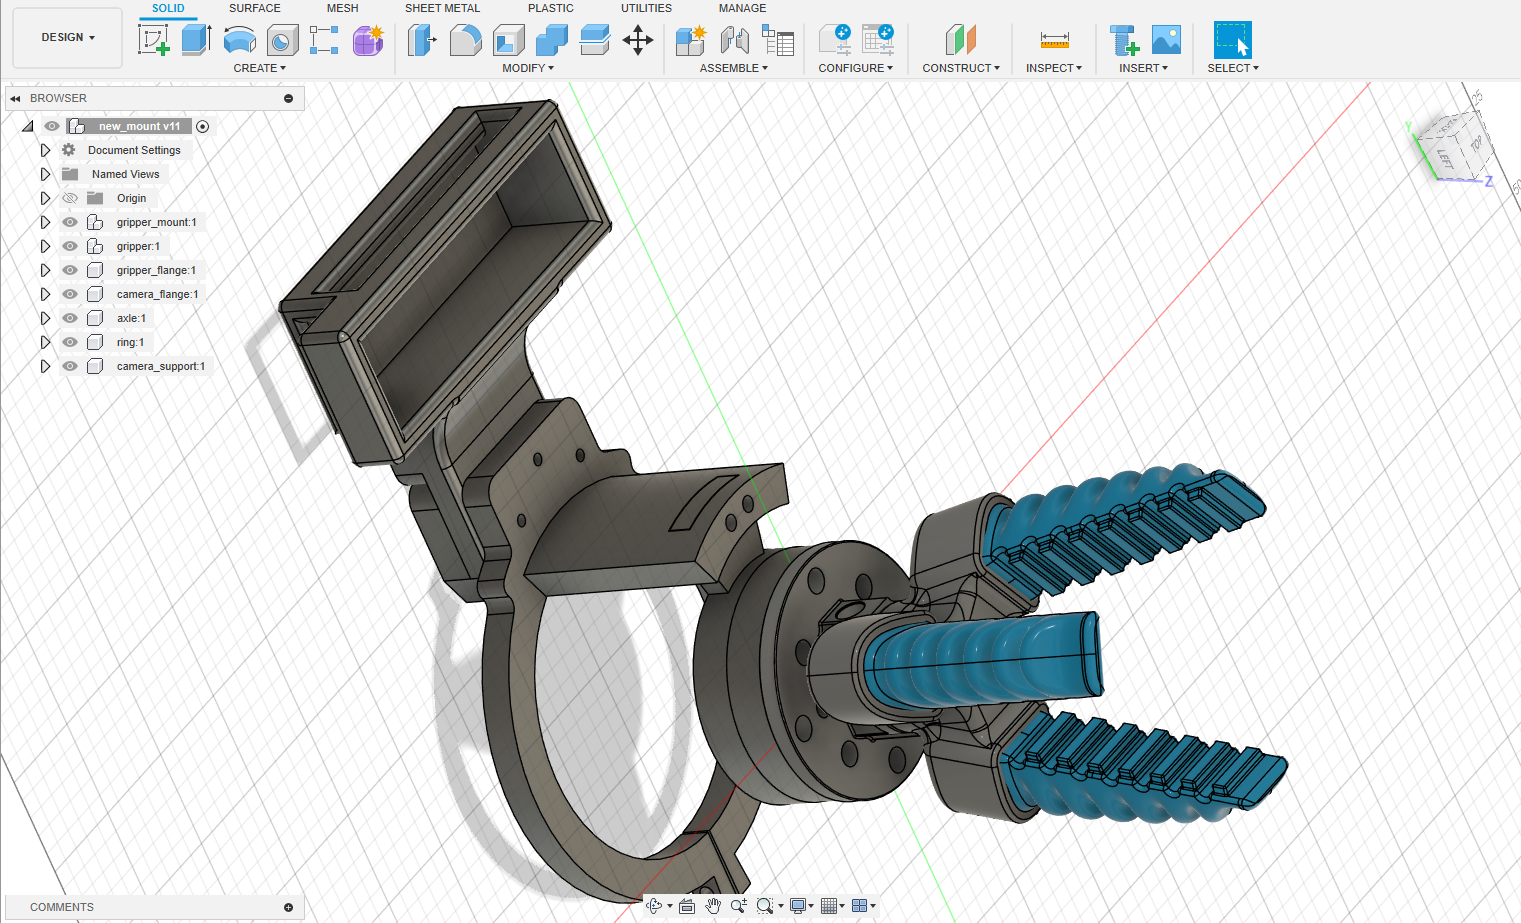
\includegraphics[width=\textwidth]{c3_24.png} % Replace with your image file
        \caption{Side view of the 3D design}
        \label{fig:sidev2}
    \end{subfigure}

    \caption{MountV2 Design screenshots from \textit{Autodesk Fusion 360}}
    \label{fig:mountv2}
\end{figure}

The second version of the mount, alias \textit{Mount V2}, was designed to be compact, robust, and more effective
for the final versions of the project and the "soft grasping" demos. The mount,
shown in \ref{fig:mountv2}, comprises 3 parts:
the flange connector, the camera mount, and the soft gripper mount. The flange connector is used to connect
the mount to the cobot's flange, ensuring that the mount is securely attached to the cobot. The camera mount
is used to mount the stereo camera on top of the cobot's wrist, ensuring that the camera has a wider field of view.
The soft gripper mount is used to mount the soft gripper on the cobot's flange connector, allowing the cobot's
end effector to grasp and manipulate objects in the environment.

The \textbf{flange connector} was designed from scratch because the flange provided by the cobot's manufacturer was not
compatible with the soft gripper mount. The flange connector was designed to be lightweight and compact, 
to ensure that the 3d printing process would be fast and structurally sound. The flange connector was also designed
to be robust and durable, to withstand the vibrations and shocks of the cobot's movements.
The camera mount is designed to be attached to the flange connector on the cobot's wrist with screws and bolts,
ensuring that the camera is securely attached to the cobot while preventing vibrations that could
offset the sensor position and orientation. The camera mount is designed to host the camera cable angled connector.
This angled connector is magnetic, and it prevents the cable from being pulled out of the camera when
the cobot's end effector moves around. This was a critical feature, set to avoid the camera's cable
being broken or damaging the internal USB-C port of the stereo camera. The MountV2 installed on the cobot
is shown in \ref{fig:c3_img17}.

\begin{figure}[t]
    \centering
    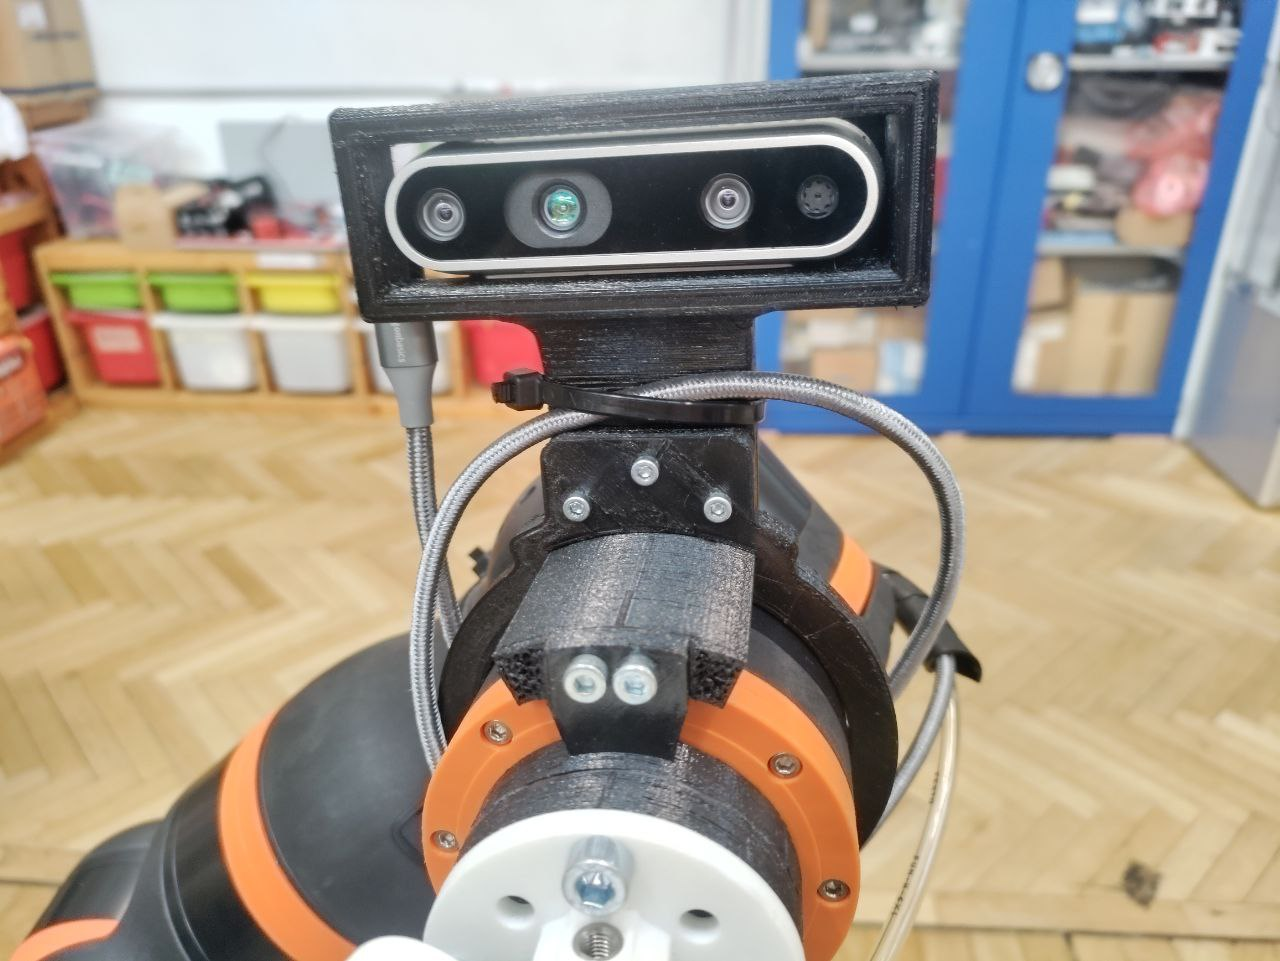
\includegraphics[width=0.6\textwidth]{c3_17.jpg}
    \captionsetup{width=1\linewidth}
    \caption{3d-printed mountV2 on the arm's wrist}.
    \label{fig:c3_img17}
\end{figure}

\subsection{Issues with the laboratory's 3D printer}

The 3D printer in the AIRLab is a printer that is used by many researchers and students for their projects.
In the past, very little maintenance was done on the printer, and the printer was not calibrated correctly.
This caused many issues with the 3D prints, such as \textbf{stringing, and under-extrusion}, which affected negatively 
the quality of my prints. Therefore I had to carry out maintenance on the printer to fix these issues.
I calibrated the printer's bed and the extruder, to ensure that the prints were of high quality and accurate.
I substituted the nozzle with a new one, and unclogged the hotend, to ensure that the filament was extruded correctly
and in the right amount. I also cleaned the printer's bed and the extruder, to ensure that the prints were sticking
correctly to the bed. After these maintenance operations, the printer was working correctly, and the prints were of
higher quality, even though they were still far from being perfect. I was not able to clean the printer's
extruder gears and the filament feeder, as they were not accessible to me due to some screws being stripped.

\section{Batteries and Power Management}

The mobile robot's internal battery is capable of powering all the sensors and computational
units that are mounted. To meet the specific voltage and current requirements of these devices, 
two DC/DC converters are employed, one of which is shown in \ref{fig:c3_img03}:

\begin{itemize}
    \item one DC/DC converter with an output voltage of 12V at a maximum of 15A for the on-board computer, router, and switch
    \item one DC/DC converter with an output voltage of 24V at a maximum of 5A for the LiDAR sensor.
\end{itemize}

The mobile robot platform's internal batteries are not sufficient to power the robotic arm and the pneumatic pump
mounted on board. To power these devices, an external power supply is used, which provides 24V at a maximum of 10A.
The cobot is powered by two 12V \textbf{lead batteries} \ref{fig:c3_img15} with 9Ah of power capacity, 
which provides the necessary power to the robotic arm motors and the pneumatic pump. 
The batteries are mounted and secured on the robot's base,
ensuring that the robot is powered and operational during its missions. There are 2 batteries available
in the laboratory, which can be switched easily when one of them is discharged.

% Add a picture of the batteries
\begin{figure}[t]
    \centering
    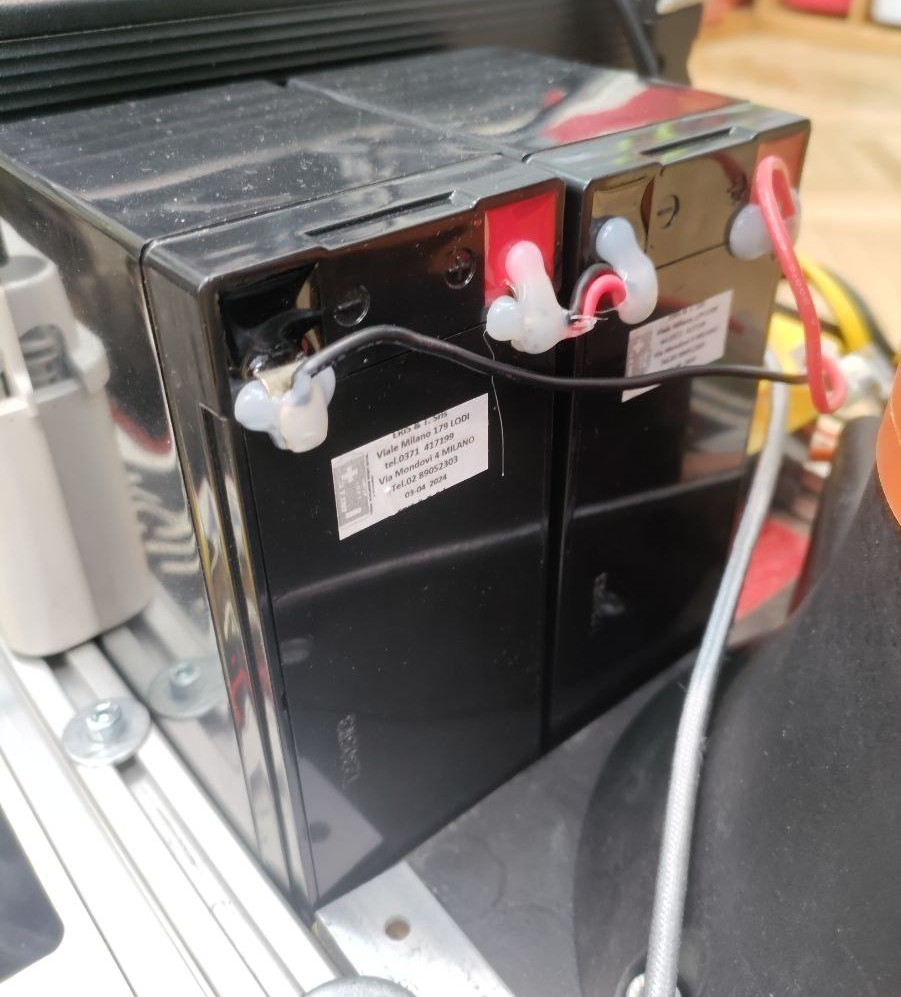
\includegraphics[width=0.5\textwidth]{c3_15.jpg}
    \captionsetup{width=1\linewidth}
    \caption{Lead batteries mounted onboard for the cobot and pneumatic pump}.
    \label{fig:c3_img15}
\end{figure}

% Add image of DC/DC converters
\begin{figure}[t]
    \centering
    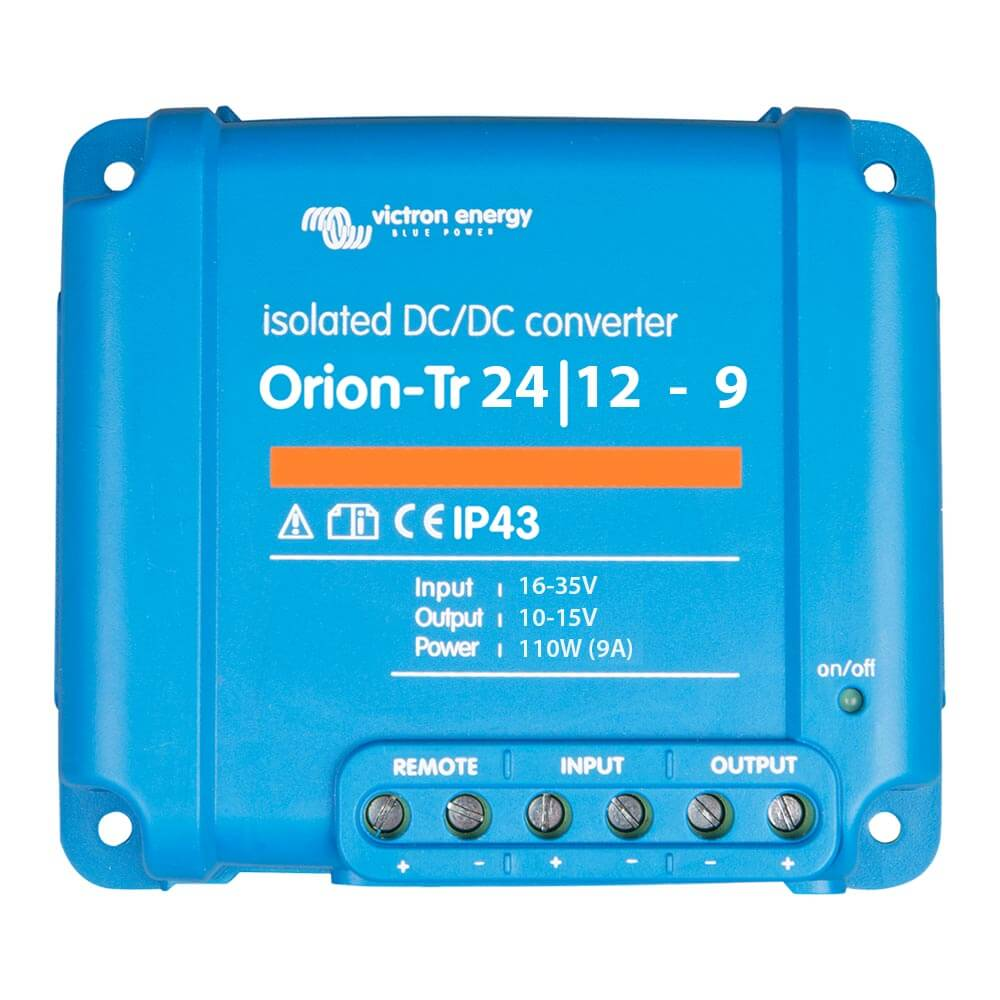
\includegraphics[width=0.4\textwidth]{chapter3_03.jpg}
    \captionsetup{width=1\linewidth}
    \caption{DC/DC converter used to power the robot's sensors and computer}.
    \label{fig:c3_img03}
\end{figure}

Another tool used to power the robots is a \textit{Santino}, a holy figure card presenting \textit{Saint Staianet}, 
the patron saint and protector of the mobile manipulation robot. This figure, placed in the front, as shown in \ref{fig:c3_img19},
helped and protected the robot during the development and testing of the project, ensuring that everything
was working fine and smoothly. The Santino was also used to provide a spiritual and religious touch to the project,
ensuring that the robot was blessed and protected during its missions.

\begin{figure}[t]
    \centering
    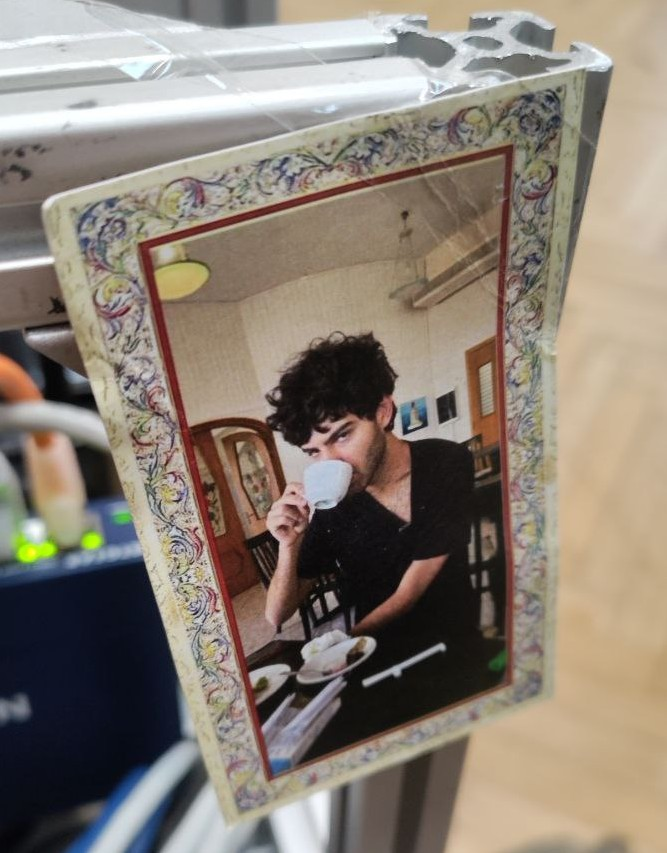
\includegraphics[width=0.5\textwidth]{c3_19.jpg}
    \captionsetup{width=1\linewidth}
    \caption{Santino}.
    \label{fig:c3_img19}
\end{figure}

\section{Complete Mobile Manipulation Setup}

Figures \ref{fig:c3_img28} and \ref{fig:c3_img29} show the complete mobile manipulation setup, with the robotic arm
mounted on top of the SCOUT 2.0 robot, and the soft gripper mounted on the robotic arm's end effector.
The setup is ready for the "soft grasping" demos, where the robot is tasked with grasping and manipulating objects
in simulated agricultural environments.

\begin{figure}[t]
    \centering
    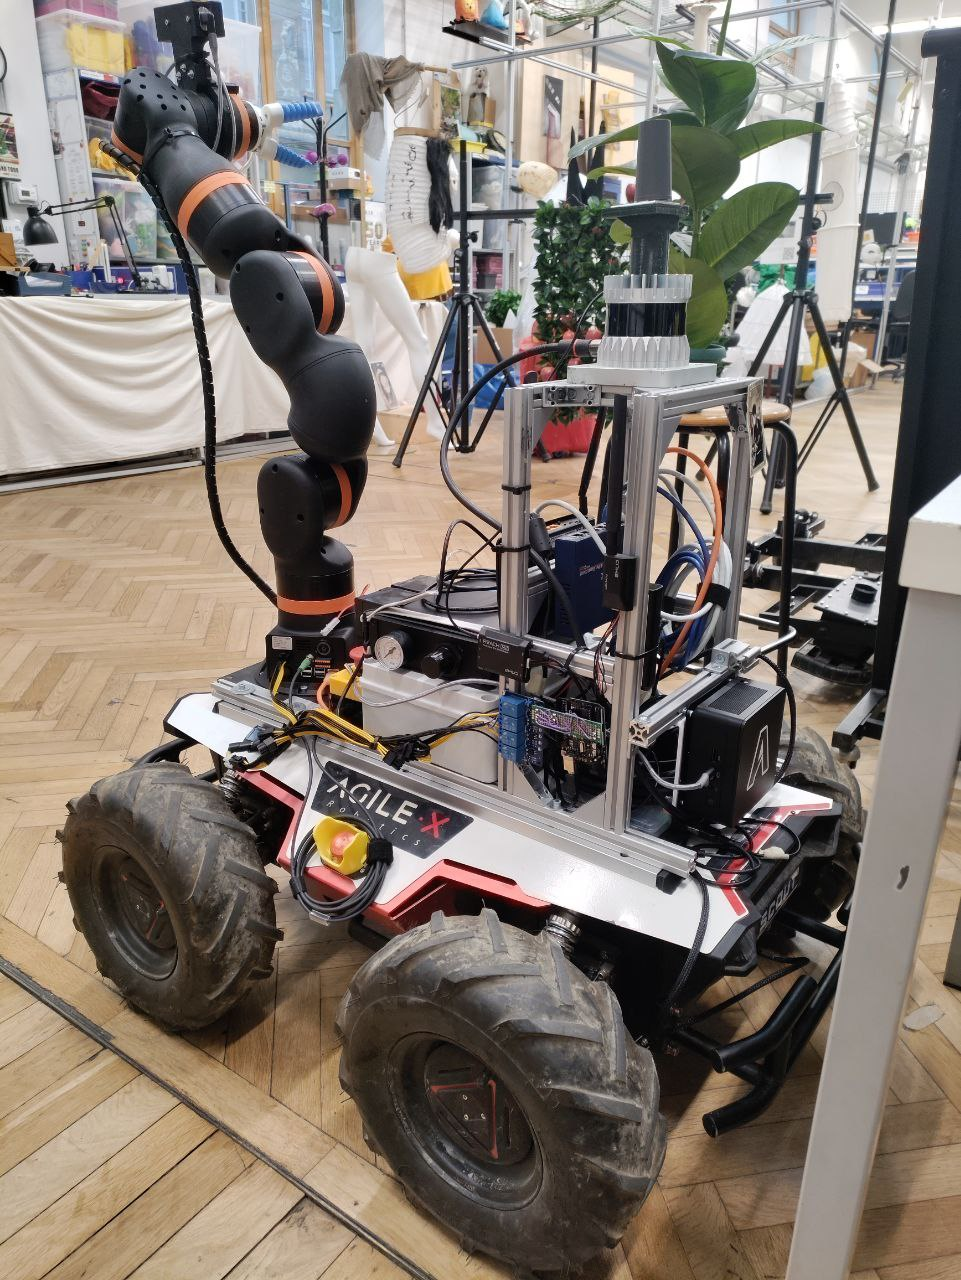
\includegraphics[width=0.8\textwidth]{c3_29.jpg}
    \captionsetup{width=1\linewidth}
    \caption{Front view of the robots}.
    \label{fig:c3_img29}
\end{figure}

\begin{figure}[t]
    \centering
    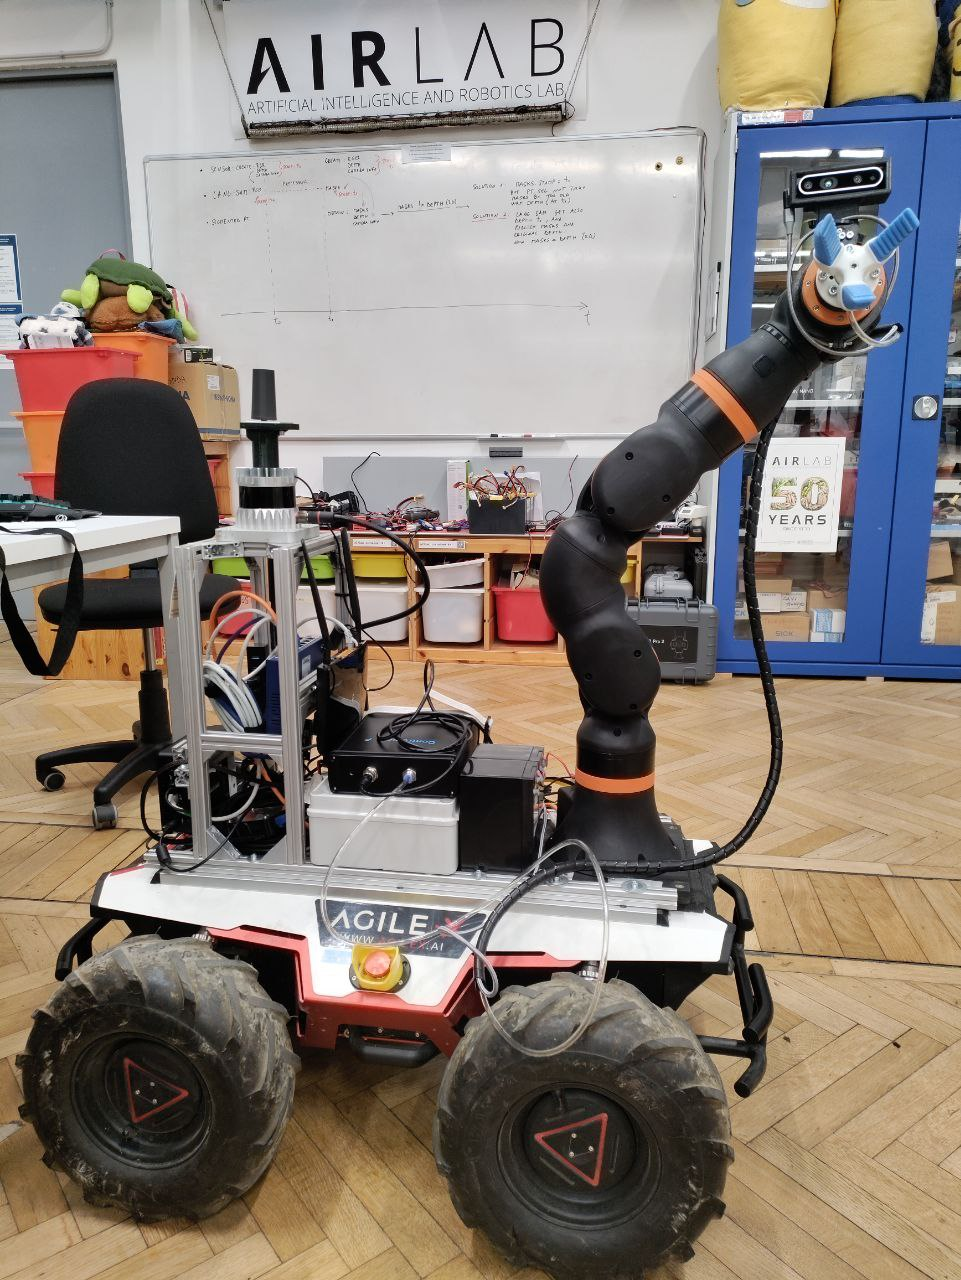
\includegraphics[width=0.8\textwidth]{c3_28.jpg}
    \captionsetup{width=1\linewidth}
    \caption{Lateral view of the robots}.
    \label{fig:c3_img28}
\end{figure}

\addtocontents{toc}{\vspace{2em}} % Add a gap in the Contents, for aesthetics

%bibtex bibliography
%\bibliography{chapters/biblio}

%biblatex bibliography
\setlength\bibitemsep{0.5\baselineskip}
\printbibliography



\end{document}